%%%%%%%%%%%%%%%%%%%%%%%%%%%%%%%%%%%%%%%%%%%%%%%%%%%%%%%%%%%%%%%%%%%%%%%%%%%%%%%%%%%%
% Document data
%%%%%%%%%%%%%%%%%%%%%%%%%%%%%%%%%%%%%%%%%%%%%%%%%%%%%%%%%%%%%%%%%%%%%%%%%%%%%%%%%%%%
\documentclass[12pt]{article} %report allows for chapters
%%%%%%%%%%%%%%%%%%%%%%%%%%%%%%%%%%%%%%%%%%%%%%%%%%%%%%%%%%%%%%%%%%%%%%%%%%%%%%%%%%%%
\usepackage{preamble}

\begin{document}

\begin{center}
   \textsc{\large MATH 271, Worksheet 1, \emph{Solutions}}\\
   \textsc{Complex Numbers}
\end{center}
\vspace{.5cm}

\begin{problem}
Add and multiply all possible pairs of the complex numbers
\[
z_1 = 3-2i \qquad z_2 = -1-i \qquad z_3 = \frac{1}{\sqrt{2}}+\frac{i}{\sqrt{2}} \qquad z_4 = -\pi + \pi i.
\]
\end{problem}

\begin{solution}
What are all the possible pairs? They are,
\begin{align*}
    z_1 z_2, \quad z_1 z_3, \quad z_1 z_4;\\
    z_2 z_3, \quad z_2 z_4;\\
    z_3 z_4.
\end{align*}
Which is $\binom{4}{2}$ (4 choose 2) options if you care!

We can then add them component by component just like when we add polynomials (specifically monomials). Here's the first one done out.
\[
z_1+z_2=(3-2i)+(-1-i)=3-1+(-2-1)i=2-3i.
\]
And the rest,
\begin{align*}
    z_1 + z_2=2-3i, \quad z_1 + z_3=\left(3+\frac{1}{\sqrt{2}}\right)+\left(-2+\frac{1}{\sqrt{2}}\right)i, \quad z_1 + z_4=(3-\pi)+(-2+\pi)i;\\
    z_2+ z_3= \left(-1+\frac{1}{\sqrt{2}}\right) + \left(-1+\frac{1}{\sqrt{2}}\right), \quad z_2 + z_4 = (-1-\pi)+(-1+\pi)i;\\
    z_3+z_4=\left(\frac{1}{\sqrt{2}}-\pi\right)+\left(\frac{1}{\sqrt{2}}+\pi\right)i.
\end{align*}

Let us multiply these. Remember, we foil these products out just like multiplying polynomials. I'll do the first one out.
\begin{align*}
    z_1z_2 = (3-2i)(-1-i)=-3+2i-3i+2i^2=-5 -i.
\end{align*}
For the rest, we have
\begin{align*}
    z_1 z_2= -5-i, \quad z_1 z_3=\frac{5}{\sqrt{2}}+\frac{i}{\sqrt{2}}, \quad z_1 z_4=-\pi +5\pi i;\\
    z_2 z_3=-\sqrt{2}i, \quad z_2 z_4=2\pi;\\
    z_3 z_4=-\sqrt{2}\pi.
\end{align*}
\end{solution}

\hrule

\begin{problem}
Plot and label the above points on the graph below. Pick two points and draw their sum geometrically. 
        \begin{center}
        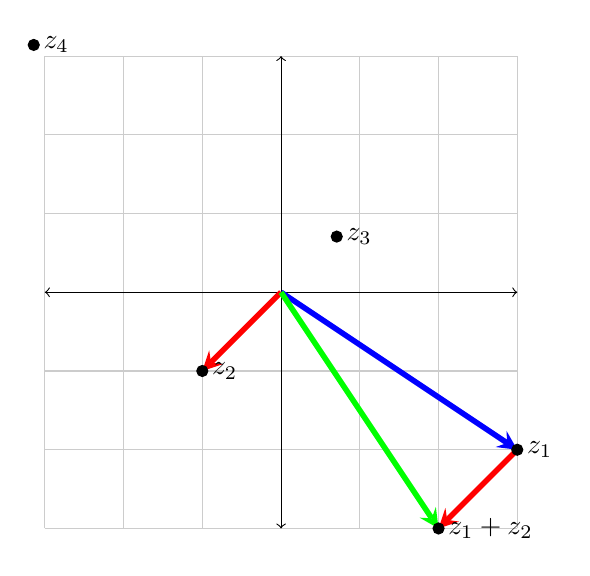
\begin{tikzpicture}
        \draw[thin,gray!40] (-3,-3) grid (3,3);
        \draw[<->] (-3,0)--(3,0) node[right]{$\RE$};
        \draw[<->] (0,-3)--(0,3) node[above]{$\IM$};
        \draw[line width=2pt,blue,-stealth](0,0)--(3,-2) node[anchor=south] at (2,-1){};
        \draw[line width=2pt,red,-stealth](0,0)--(-1,-1) node[anchor=east] at (1,-2){};
        \draw[line width=2pt,red,-stealth](3,-2)--(2,-3) node[anchor=east] at (2,-1){};
        \draw[line width=2pt,green,-stealth](0,0)--(2,-3) node[anchor=east] at (2,-1){};
        \foreach \Point/\PointLabel in {(3,-2)/z_1, (-1,-1)/z_2, (.707,.707)/z_3, (-3.141,3.141)/z_4, (2,-3)/{z_1+z_2}}
        \draw[fill=black] \Point circle (0.07) node[right] {$\PointLabel$};
        \end{tikzpicture}
        \end{center}
\end{problem}

\begin{solution}
I'll use the above graph. I'll pick $z_1$ and $z_2$ to add.
\end{solution}
\hrule

\begin{problem}
Convert all the above complex numbers in Cartesian form to polar form.
\end{problem}

\begin{solution}
Recall that given
\[
z=a+bi,
\]
then for $a>0$ we have
\[
\theta = \arctan\left(\frac{b}{a}\right) \qquad \textrm{and} \qquad r = \sqrt{zz^*}=\sqrt{a^2+b^2},
\]
and for $a<0$ we have
\[
\theta = \arctan\left(\frac{b}{a}\right) + \pi.
\]
Thus, 
\begin{align*}
z_1 &\approx  \sqrt{13}e^{-0.588i},\\
z_2 &= -\sqrt{2}e^{i\frac{\pi}{4}}=\sqrt{2}e^{i\frac{5\pi}{4}},\\
z_3 &= e^{i\frac{\pi}{4}}\\
z_4 &= \pi \sqrt{2}e^{i\frac{3\pi}{4}}.
\end{align*}
\end{solution}

\hrule

\begin{problem}
Multiply all possible pairs of complex numbers
\[
w_1 = e^{i\pi} \qquad w_2 = -\sqrt{2} e^{i\frac{\pi}{4}} \qquad w_3 = 2 e^{-i\frac{\pi}{3}} \qquad w_4= 3 e^{i\frac{\pi}{2}}.
\]
\end{problem}

\begin{solution}
We have
\begin{align*}
    w_1 w_2 = -\sqrt{2}e^{i\frac{5\pi}{4}}, \quad w_1 w_3 = 2e^{i\frac{2\pi}{3}}, \quad w_1 w_4 = 3 e^{i\frac{3\pi}{2}};\\
    w_2 w_3 = -2\sqrt{2}e^{-i\frac{\pi}{12}}, \quad w_2 w_4 =-3\sqrt{2}e^{i\frac{3\pi}{4}};\\
    w_3 w_4 = 6 e^{i\frac{\pi}{6}}.
\end{align*}
\end{solution}

\hrule

\begin{problem}
Plot and label the above points in the graph below.  Draw the product $w_1w_2$ geometrically.
        \begin{center}
            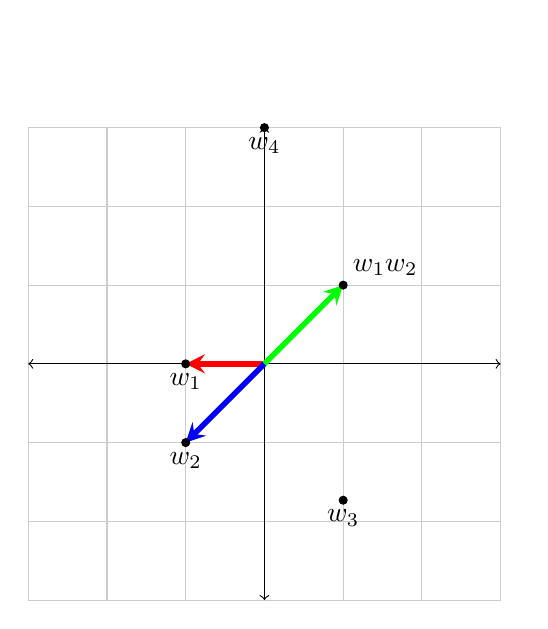
\begin{tikzpicture}
            \draw[thin,gray!40] (-3,-3) grid (3,3);
            \draw[<->] (-3,0)--(3,0) node[right]{$\RE$};
            \draw[<->] (0,-3)--(0,3) node[above]{$\IM$};
            \tdplotdrawarc[->,line width = 1pt, black]{(0,0)}{1}{0}{180}{}{};
            \node[anchor=east] at (-.75,1){};
            \tdplotdrawarc[->,line width = 1pt, black]{(0,0)}{1.3}{0}{405}{}{};
            \node[anchor=west] at (1.4,.5){};
            \tdplotdrawarc[->,line width = 1pt, black]{(0,0)}{.5}{0}{225}{}{};
            \node[anchor=north east] at (-1,-1){};
            \draw[line width=2pt,red,-stealth](0,0)--(-1,0) node[anchor=south east] at (0,4){};
            \draw[line width=2pt,blue,-stealth](0,0)--(-1,-1) node[anchor=south east] at (2.828,2.828){};
            \draw[line width=2pt,green,-stealth](0,0)--(1,1) node[anchor=south west] at (1,1){};
            \node[anchor=south west] at (1,1){$w_1 w_2$};
            \draw[fill=black] (1,1) circle (0.05);
            \foreach \Point/\PointLabel in {(-1,0)/w_1, (-1,-1)/w_2, (1,-1.732)/w_3, (0,3)/w_4}
            \draw[fill=black] \Point circle (0.05) node[below] {$\PointLabel$};
            \end{tikzpicture}
        \end{center}
\end{problem}

\begin{solution}
I'll use the above graph.
\end{solution}

\hrule 
\begin{problem}
Show by a geometrical argument that $re^{i\theta}=re^{i(\theta+2n\pi)}$ for any integer value of $n$.  Can you also show this by the typical conversion from polar to Cartesian?
\end{problem}

\begin{solution}
By considering $\theta+2n\pi$ we are looking at rotating the same number by an integer copy of $2\pi$. Since rotation by $2\pi$ takes us all the way around to where we start from, any rotation of an integer times this amount will also take us back to where we started. Thus, we can say $re^{i\theta}=re^{i(\theta+2n\pi)}$. 

Yes, we can. $\cos$ and $\sin$ are both $2\pi$ periodic and thus we can just write
\[
a=r\cos(\theta)=r\cos(\theta+2n\pi)
\]
and
\[
b=r\sin(\theta)=r\sin(\theta+2n\pi).
\]
\end{solution}

\hrule

\begin{problem}
Let $z=a+bi$.  What is $z^*?$  What is $z$ in polar coordinates? How about $z^*$? Can you explain why $zz^*$ will always be real using a geometrical (polar coordinate) argument?
\end{problem}

\begin{solution}
$z^*$ is the complex conjugate and $z^*=a-bi$.  We can write $z=re^{i\theta}$ for a polar coordinate representation of $z$.  In polar coordinates, we then have $z^*=re^{-i\theta}$. $zz^*$ will always be real since multiplication of two complex numbers with opposing angles will have a resulting angle of $0$. This is exactly a real number. That is, see
\[
\left( re^{i\theta} \right) \left(re^{-i\theta}\right) = r^2.
\]
\end{solution}

\hrule

\begin{problem}
Show that the functions $\sin(x)$ and $\cos(x)$ are periodic and determine the period.  Is the function $\tan(x)$ periodic?
\end{problem}

\begin{solution}
Showing that $\sin(x)$ and $\cos(x)$ are periodic relies on us knowing the period.  We have used these functions quite often, and know that they repeat themselves after $2\pi$. One can simply check by graphing or with a calculator that we always have
\[
\sin(x)=\sin(x+2\pi) \qquad \textrm{and} \qquad \cos(x)=\cos(x+2\pi).
\]
Yes, $\tan(x)$ is periodic.  It has period $\pi$.
\end{solution}


\hrule 
\begin{problem}
(Roots of unity) Given that $i^2=-1$ we can factor equations in ways that are totally new to us.  Solve the following. Geometrical reasoning may really help you here!
\begin{enumerate}[(a)]
    \item Find all solutions to $z^2=1$.
    \item Find all solutions to $z^3=1$.
    \item Find all solutions to $z^4=1$.
    \item *Find all solutions to $z^n=1$.
\end{enumerate}
\emph{Hint: each of the above has $n$ solutions for $z^n$.}
\end{problem}

\begin{solution}
Think about using rotations to answer this question.  I'll try to phrase that here. You should also plot these to see the symmetry!
\begin{enumerate}[(a)]
    \item There will be two complex solutions of $z^2=1$ since it is a degree two polynomial.  Now, what we are asking for are numbers of length one such that when we double there angle (squaring a complex number does this) we get $2n\pi$ for any integer $n$.  So we can divide $2\pi$ by two and get $\pi$. Our solutions are
    \[
    -1=e^{i\pi} \qquad \textrm{and} 1=e^{i2\pi}.
    \]
    \item There will be three complex solutions. We need angles that triple to give us $2n\pi$.  So we can take angles $2\pi/3$, $4\pi/3$ and $2\pi$ to get solution. Thus,
    \[
    e^{i\frac{2\pi}{3}}, \qquad e^{i\frac{4\pi}{3}}, \qquad e^{i2\pi}
    \]
    are solutions.
    \item There will be four complex solutions. We have solutions
    \[
    e^{i\frac{\pi}{2}}, \qquad e^{i\pi}, \qquad e^{i\frac{3\pi}{4}}, \qquad e^{i2\pi}.
    \]
    \item There will be $n$ complex solutions of the form
    \[
    e^{i\frac{2k\pi}{n}} \qquad \textrm{where $k=0,1,\dots,n-1$}.
    \]
\end{enumerate}
\end{solution}


\hrule
\begin{problem}
(Rotational symmetries) Consider a complex number $z=a+bi=re^{i\theta}$. What happens to this point as we repeatedly multiply by $i$? Pick a specific $z$ (i.e., fix $a$ and $b$ or $r$ and $\theta$) and multiply by $i$ until you see a pattern.  What is happening? \emph{Note: this is an example of a symmetry group or a discrete dynamical system!}
\end{problem}

\begin{solution}
Let's do this in Cartesian form first.
\begin{align*}
    z &= a+bi\\
    iz &= -b+ai\\
    i^2z &= -a-bi\\
    i^3z &= b-ai\\
    i^4z &= z.
\end{align*}
The pattern continues from there. The original point comes back to where it started after four iterations. 

Considering polar coordinates, $i=e^{i\frac{\pi}{2}}$, which tells us that multiplication by $i$ is simply rotation by $\frac{\pi}{2}$.
\end{solution}


\hrule 
\begin{problem}
(Why $i$?) Consider the following (differential) equation
\[
\frac{d^2}{dt^2}x(t)=-x(t).
\]
Now, let $x(t)=e^{it}$.  Show that the above expression is true.
\end{problem}

\begin{solution}
Indeed, we take
\[
x'(t)=ie^{it}
\]
and
\[
x''(t)=i\left(ie^{it}\right)=-e^{it}=-x(t).
\]
\end{solution}

\hrule

\begin{problem}
(Characteristic polynomial) Consider the following (differential) equation
\[
ax''(t)+bx'(t)+cx(t)=0.
\]
This equation can be converted to a quadratic equation
\[
a\lambda^2 + b\lambda + c = 0.
\]
What are the roots to this equation?
\end{problem}

\begin{solution}
This is just asking for the quadratic formula which states
\[
\lambda = \frac{-b\pm \sqrt{b^2-4ac}}{2a}.
\]
This will be important for us in the future. This is why we need complex numbers!
\end{solution}


\hrule
\begin{problem}
(Bonus) The complex numbers can be thought of as a 2-dimensional number system. The \textbf{quaternions} are a 4-dimensional number system that are of the form
\[
q = a+bi+cj+dk.
\]
We define $i^2=j^2=k^2=ijk=-1$. Pick another quaternion $\tilde{q}=\tilde{a}+\tilde{b}i+\tilde{c}j+\tilde{d}k$ and multiply each together. Is multiplication commutative? \emph{Note: quaternions are extremely useful in 3-dimensional systems. They are used for computer graphics or for formalizing the vector calculus in $\R^3$ which we will see in Math 272.}
\end{problem}

\begin{solution}
I'll let you read about this more on your own!
\end{solution}

\end{document}
